\subsection{Solving Puzzles}


On \verb'puzzles.com', we find the following checkerboard puzzle:
\begin{quote}
Rearrange the six pieces so that to form the $5\times 5$ 
checkerboard shown in the center of the illustration.
\end{quote}
The following illustration goes along with it:
$$
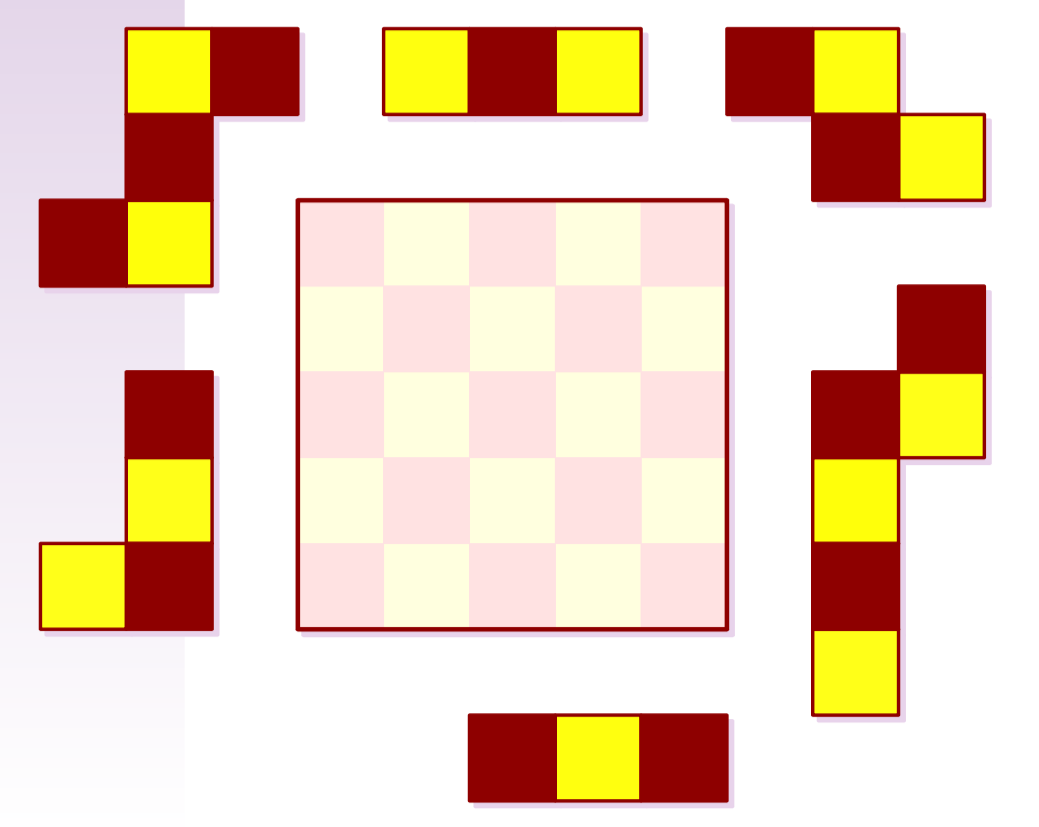
\includegraphics[width=90mm]{GRAPHICS/checkerboard_puzzle}
$$
We wish to write a program to solve this puzzle for us. 
The way we approach this problem is the following. 
We wish to express the required conditions  
as a system of equation. The variables in the system correspond to the pieces in the various positions. 
The equations in the system capture the condition that each spot on the checkerboard 
is occupied by exactly one piece 
and that each piece is used exactly once. 
We label the $25$ spots using the integers $0$ through $24$ in the following way:
$$
\begin{array}{|c|c|c|c|c|}
\hline
0 & 1 & 2 & 3 & 4 \\
\hline
5 & 6 & 7 & 8 & 9 \\
\hline
10 & 11 & 12 & 13 & 14 \\
\hline
15 & 16 & 17 & 18 & 19 \\
\hline
20 & 21 & 22 & 23 & 24 \\
\hline
\end{array}
$$
The conditions lead to a system of equations 
$$
A \bx = \bone
$$
where $A$ is a matrix over $\{0,1\}$ and $\bx$ is a $\{0,1\}$-vector. 
The right hand side is the all-one vector.
A piece in a certain position will be identified with the spots that it covers. 
That way, pieces in positions become subsets of the set $\{0,\ldots,24\}.$
In order to obtain all possible positions of a piece, we start by putting the piece in the upper left corner 
of the board, making sure that the colors match. Once this is done, we record the translation vectors 
that are allowed. 
A translation vector is simply an integer that can be added to the set so that the 
resulting set is the set of spots occupied by the moved piece. 
A piece can also be rotated. 
We record the 
4 rotations using the integers $\{0,1,2,3\}.$ 
Once all translations and rotations are defined, we set up the coefficient matrix $A$. 
The first 25 rows of $A$ are the conditions that each spot on the board is occupied by exactly one piece.  
Then, we add 6 more rows to $A$, each row corresponding to an equation that ensures that a certain piece 
is chosen exactly once.
Once the system $A$ has been computed, we store it on file. 
Here is the code:


{\small
{\tt
\input CODE/puzzle.tex
}
}

Here is the output of the program (slightly cut in order to save space). At the bottom, we see the matrix $A$.

{\scriptsize
{\tt
\input CODE/puzzle_out_edited.tex
}
}

The file \verb'puzzle25_compressed.txt' is this:

{\scriptsize
{\tt
\input CODE/puzzle25_compressed.tex
}
}

The program \verb'dlx.out' takes this file and solves the associated system $A \bx = \bone.$ The solutions are written to 
yet another file. There are exactly four solutions:

{\tt
\input CODE/sol25.tex
}
The four solutions are essentially all one and the same solution. 
This one solution appears in all $4$ different rotations.
$$
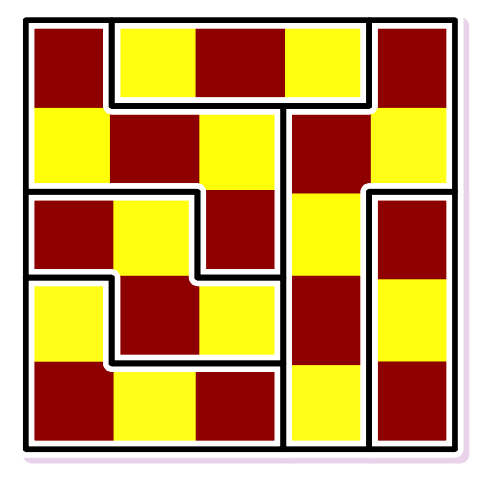
\includegraphics[width=45mm]{GRAPHICS/checkerboard_solution}
$$
The program \verb'dlx.out' performs a backtrack search. 
The search tree looks as follows. Each node corresponds to 
one state of the variable $\bx$ that is examined.
$$
\input GRAPHICS/puzzle25_search.tex
$$
The four deep branches correspond to the four solutions.
Altogether, the search examines 63 nodes.

